\chapter{Specifikacija programske potpore}
		
	\section{Funkcionalni zahtjevi}
			
			%\textbf{\textit{dio 1. revizije}}\\
			
%			\textit{Navesti \textbf{dionike} koji imaju \textbf{interes u ovom sustavu} ili  \textbf{su nositelji odgovornosti}. To su prije svega korisnici, ali i administratori sustava, naručitelji, razvojni tim.}\\
%				
%			\textit{Navesti \textbf{aktore} koji izravno \textbf{koriste} ili \textbf{komuniciraju sa sustavom}. Oni mogu imati inicijatorsku ulogu, tj. započinju određene procese u sustavu ili samo sudioničku ulogu, tj. obavljaju određeni posao. Za svakog aktora navesti funkcionalne zahtjeve koji se na njega odnose.}\\
			
			
			\noindent \textbf{Dionici:}
			
			\begin{packed_enum}
				
				\item Korisnici (učenici)
				\item Administrator riječi				
				\item Razvojni tim
				\item Konkurencija
				\item Naručitelj
				
			\end{packed_enum}
			
			\noindent \textbf{Aktori i njihovi funkcionalni zahtjevi:}
			
			
			\begin{packed_enum}
				\item  \underbar{Korisnik može:}
				
				\begin{packed_enum}
					
					\item registrirati se
					\item prijaviti se
					\item odjaviti se
%					\begin{packed_enum}
%						
%						\item  podfunkcionalnost 1 
%						\item  podfunkcionalnost 2
%				
%					\end{packed_enum}
					\item odabrati rječnik i mod učenja
					\item odgovarati na pitanja
					\item obrisati svoj korisnički račun
					
				\end{packed_enum}
			
				\item  \underbar{Administrator riječi može:}
				
				\begin{packed_enum}
					
					\item dodati riječ u rječnik
					\item urediti komponente riječi
					\item ukloniti riječ iz baze
					\item kreirati novi rječnik
					\item obrisati rječnik
					\item dodati novog administratora
										
				\end{packed_enum}
			\end{packed_enum}
			
			\eject 
			
			
				
			\subsection{Obrasci uporabe}
				
% {dio 1. revizije}}
				
				\subsubsection{Opis obrazaca uporabe}
%{Funkcionalne zahtjeve razraditi u obliku obrazaca uporabe. Svaki obrazac je potrebno razraditi prema donjem predlošku. Ukoliko u nekom koraku može doći do odstupanja, potrebno je to odstupanje opisati i po mogućnosti ponuditi rješenje kojim bi se tijek obrasca vratio na osnovni tijek.}
					


					\noindent \underbar{\textbf{UC1 - Registracija}}
					\begin{packed_item}
	
						\item \textbf{Glavni sudionik: } Korisnik
						\item  \textbf{Cilj:} 
						\item  \textbf{Sudionici:} Backend
						\item  \textbf{Preduvjet:} -
						\item  \textbf{Opis osnovnog tijeka:}  
						
						\item[] \begin{packed_enum}
	
							\item Korisnik odabire opciju registracija
							\item Sustav prikazuje formu za unos podataka (ime, email,...)
							\item Korisnik unosi podatke i potvrđuje registraciju
							\item Sustav pohranjuje podatke i šalje email s inicijalnom lozinkom
							
						\end{packed_enum}
						
						\item  \textbf{Opis mogućih odstupanja:}
						
						\item[] \begin{packed_item}
	
							\item[3.a] Korisnik odustaje od registracije
							\item[] \begin{packed_enum}
								
								\item Sustav se vraća na početnu stranicu
								
							\end{packed_enum}
							\item[4.a] U sustavu već postoji korisnik s istom email adresom
							\item[] \begin{packed_enum}
								
								\item Sustav obaviještava korisnika da se email adresa već koristi
								
							\end{packed_enum}
							\item[4.b] Nevažeća email adresa
								% Što tada? Hoćemo li realizirati provjeru email adrese i obaviještavanje korisnika u slučaju da je nevažeća ili ne?

						\end{packed_item}
					\end{packed_item}
					
					
					\noindent \underbar{\textbf{UC2 - Prijava}}
					\begin{packed_item}
						
						\item \textbf{Glavni sudionik: } Korisnik
						\item  \textbf{Cilj:} 
						\item  \textbf{Sudionici:} Backend
						\item  \textbf{Preduvjet:} UC1(Registracija)
						\item  \textbf{Opis osnovnog tijeka:}
						
						\item[] \begin{packed_enum}
							
							\item Korisnik odabire opciju prijava
							\item Sustav prikazuje formu za unos podataka
							\item Korisnik unosi podatke i potvrđuje prijavu
							\item Sustav otvara stranicu s ponuđenim jezicima
						\end{packed_enum}
						
						\item  \textbf{Opis mogućih odstupanja:}
						
						\item[] \begin{packed_item}
							
							\item[3.a] Korisnik odustaje od prijave
							\item[] \begin{packed_enum}
								
								\item Sustav prikazuje početnu stranicu
								
							\end{packed_enum}
							
							\item[3.b] Uneseni podatci za prijavu su netočni
							\item[] \begin{packed_enum}
								
								\item Sustav obaviještava korisnika da su uneseni podatci netočni
								
							\end{packed_enum}
							
							\item[3.c] Korisnik se prijavljuje po prvi put
							\item[] \begin{packed_enum}
								
								\item Sustav prikazuje formu za promijenu lozinke
								
							\end{packed_enum}
							
							
						\end{packed_item}
					\end{packed_item}
					
						\noindent \underbar{\textbf{UC3 - Odjava}}
					\begin{packed_item}
						
						\item \textbf{Glavni sudionik: } Korisnik
						\item  \textbf{Cilj:} 
						\item  \textbf{Sudionici:} Backend
						\item  \textbf{Preduvjet:} UC2(Prijava)
						\item  \textbf{Opis osnovnog tijeka:}
						
						\item[] \begin{packed_enum}
							
							\item Korisnik odabire opciju "Odjava"
							\item Sustav prikazuje početnu stranicu
						\end{packed_enum}
					\end{packed_item}
					
						\noindent \underbar{\textbf{UC4 - Odabir jezika}}
					\begin{packed_item}
						
						\item \textbf{Glavni sudionik: } Korisnik
						\item  \textbf{Cilj:} 
						\item  \textbf{Sudionici:} Backend
						\item  \textbf{Preduvjet:} UC2(Prijava)
						\item  \textbf{Opis osnovnog tijeka:}
						
						\item[] \begin{packed_enum}
							
							\item Korisnik odabire jezik
							\item Sustav prikazuje stranicu s odabirom rječnika
						\end{packed_enum}
						
					\end{packed_item}
					
					\noindent \underbar{\textbf{UC5 - Odabir rječnika i moda učenja}}
					\begin{packed_item}
						
						\item \textbf{Glavni sudionik: } Korisnik
						\item  \textbf{Cilj:} 
						\item  \textbf{Sudionici:} Backend
						\item  \textbf{Preduvjet:} UC4(Odabir jezika)
						\item  \textbf{Opis osnovnog tijeka:}
						
						\item[] \begin{packed_enum}
							
							\item Korisnik odabire rječnik
							\item Sustav prikazuje formu za odabir moda učenja(upit engleske riječi uz odabir hrvatskog prijevoda, upit hrvatske riječi uz odabir engleskog prijevoda, upit izgovorom engleske riječi uz odgovor pisanjem riječi na engleskom, upit tekstualnim oblikom engleske riječi uz snimanje izgovora u zvučnu datoteku)
							\item Korisnik odabire mod učenja
							\item Sustav prikazuje stranicu s prvim pitanjem
						\end{packed_enum}
						
						\item  \textbf{Opis mogućih odstupanja:}
						
						\item[] \begin{packed_item}
							
							\item[3.a] Korisnik odustaje od odabira moda
							\item[] \begin{packed_enum}
								
								\item Sustav prikazuje stranicu s odabirom rječnika
								
							\end{packed_enum}
							
							\item[4.a] Korisnik odustaje od kviza 
							\item[] \begin{packed_enum}
								
								\item Sustav prikazuje stranicu s odabirom rječnika
								
							\end{packed_enum}
							
						\end{packed_item}
					\end{packed_item}
					
					\noindent \underbar{\textbf{UC6 - Odgovor na pitanje}}
					\begin{packed_item}
						
						\item \textbf{Glavni sudionik: } Korisnik
						\item  \textbf{Cilj:} 
						\item  \textbf{Sudionici:} Backend
						\item  \textbf{Preduvjet:} UC5(Odabir rječnika i moda učenja)
						\item  \textbf{Opis osnovnog tijeka:}
						
						\item[] \begin{packed_enum}
							
							\item Korisnik daje odgovor
							\item Sustav pohranjuje odgovor i obaviještava korisnika o točnosti njegovog odgovora
							\item Korisnik odabire opciju "Nastavi"
							\item Sustav prikazuje sljedeće pitanje
						\end{packed_enum}
						
						\item  \textbf{Opis mogućih odstupanja:}
						
						\item[] \begin{packed_item}
							
							\item[3.a] Korisnik odustaje od kviza
							\item[] \begin{packed_enum}
								
								\item Sustav prikazuje stranicu s odabirom rječnika
								
							\end{packed_enum}
							
							\item[4.a] Korisnik odustaje od kviza 
							\item[] \begin{packed_enum}
								
								\item Sustav prikazuje stranicu s odabirom rječnika
								
							\end{packed_enum}
							
						\end{packed_item}
					\end{packed_item}
					
					\noindent \underbar{\textbf{UC6.1 - Odabir odgovora}}
					\begin{packed_item}
						
						\item \textbf{Glavni sudionik: } Korisnik
						\item  \textbf{Cilj:} 
						\item  \textbf{Sudionici:} Backend
						\item  \textbf{Preduvjet:} UC5(Odabir rječnika i moda učenja)
						\item  \textbf{Opis osnovnog tijeka:}
						
						\item[] \begin{packed_enum}
							
							\item Korisnik odabire jedan odgovor među ponuđenima
							\item Sustav pohranjuje odgovor i obaviještava korisnika o točnosti njegovog odgovora
							\item Korisnik odabire opciju "Nastavi"
							\item Sustav prikazuje sljedeće pitanje
						\end{packed_enum}
						
						\item  \textbf{Opis mogućih odstupanja:}
						
						\item[] \begin{packed_item}
							
							\item[3.a] Korisnik odustaje od kviza
							\item[] \begin{packed_enum}
								
								\item Sustav prikazuje stranicu s odabirom rječnika
								
							\end{packed_enum}
							
							\item[4.a] Korisnik odustaje od kviza 
							\item[] \begin{packed_enum}
								
								\item Sustav prikazuje stranicu s odabirom rječnika
								
							\end{packed_enum}
							
						\end{packed_item}
					\end{packed_item}
					
					\noindent \underbar{\textbf{UC6.2 - Unos odgovora}}
					\begin{packed_item}
						
						\item \textbf{Glavni sudionik: } Korisnik
						\item  \textbf{Cilj:} 
						\item  \textbf{Sudionici:} Backend
						\item  \textbf{Preduvjet:} UC5(Odabir rječnika i moda učenja)
						\item  \textbf{Opis osnovnog tijeka:}
						
						\item[] \begin{packed_enum}
							
							\item Korisnik unosi odgovor u polje za unos odgovora i potvrđuje klikom na gumb
							\item Sustav pohranjuje odgovor i obaviještava korisnika o točnosti njegovog odgovora
							\item Korisnik odabire opciju "Nastavi"
							\item Sustav prikazuje sljedeće pitanje
						\end{packed_enum}
						
						\item  \textbf{Opis mogućih odstupanja:}
						
						\item[] \begin{packed_item}
							
							\item[3.a] Korisnik odustaje od kviza
							\item[] \begin{packed_enum}
								
								\item Sustav prikazuje stranicu s odabirom rječnika
								
							\end{packed_enum}
							
							\item[4.a] Korisnik odustaje od kviza 
							\item[] \begin{packed_enum}
								
								\item Sustav prikazuje stranicu s odabirom rječnika
								
							\end{packed_enum}
							
						\end{packed_item}
					\end{packed_item}
					
					\noindent \underbar{\textbf{UC6.3 - Snimanje izgovora u zvučnu datoteku}}
					\begin{packed_item}
						
						\item \textbf{Glavni sudionik: } Korisnik
						\item  \textbf{Cilj:} 
						\item  \textbf{Sudionici:} Backend
						\item  \textbf{Preduvjet:} UC5(Odabir rječnika i moda učenja)
						\item  \textbf{Opis osnovnog tijeka:}
						
						\item[] \begin{packed_enum}
							
							\item Korisnik snima izgovor u zvučnu datoteku
							\item Sustav pohranjuje zvučnu datoteku i obaviještava korisnika o točnosti njegovog odgovora
							\item Korisnik odabire opciju "Nastavi"
							\item Sustav prikazuje sljedeće pitanje
						\end{packed_enum}
						
						\item  \textbf{Opis mogućih odstupanja:}
						
						\item[] \begin{packed_item}
							
							\item[3.a] Korisnik odustaje od kviza
							\item[] \begin{packed_enum}
								
								\item Sustav prikazuje stranicu s odabirom rječnika
								
							\end{packed_enum}
							
							\item[4.a] Korisnik odustaje od kviza 
							\item[] \begin{packed_enum}
								
								\item Sustav prikazuje stranicu s odabirom rječnika
								
							\end{packed_enum}
							
						\end{packed_item}
					\end{packed_item}
					
					\noindent \underbar{\textbf{UC7 - Brisanje korisničkog računa}}
					\begin{packed_item}
						
						\item \textbf{Glavni sudionik: } Korisnik
						\item  \textbf{Cilj:} 
						\item  \textbf{Sudionici:} Backend
						\item  \textbf{Preduvjet:} UC2(Prijava)
						\item  \textbf{Opis osnovnog tijeka:}
						
						\item[] \begin{packed_enum}
							
							\item Korisnik odabire opciju brisanja korisničkog računa
							\item Sustav prikazuje prozor s upitom "Jeste li sigurni da želite obrisati svoj korisnički račun?"
							\item Korisnik odabire opciju "Da"
							\item Sustav briše korisnički račun i prikazuje početnu stranicu
						\end{packed_enum}
						
						\item  \textbf{Opis mogućih odstupanja:}
						
						\item[] \begin{packed_item}
							
							\item[3.a] Korisnik odustaje od brisanja korisničkog računa
							\item[] \begin{packed_enum}
								
								\item Sustav prikazuje stranicu s odabirom rječnika
								
							\end{packed_enum}
							
						\end{packed_item}
					\end{packed_item}
					
					\noindent \underbar{\textbf{UC8 - Kreiranje novog rječnika}}
					\begin{packed_item}
						
						\item \textbf{Glavni sudionik: } Administrator riječi
						\item  \textbf{Cilj:} Kreiranje novog rječnika
						\item  \textbf{Sudionici:} Backend
						\item  \textbf{Preduvjet:} UC2 (Prijava)
						\item  \textbf{Opis osnovnog tijeka:}
						
						\item[] \begin{packed_enum}
							
							\item Administrator odabire opciju "Kreiraj novi rječnik"
							\item Sustav otvara formu za upis podataka o rječniku 
							\item Administrator upisuje sve potrebne podatke
							\item Administrator odabire opciju "Spremi"
							\item Sustav sprema promjene i prikazuje početnu stranicu
						
						\end{packed_enum}
					
						\item  \textbf{Opis mogućih odstupanja:}
					
						\item[] \begin{packed_item}
						
							\item[3.a] Administrator ne upisuje sve potrebne podatke 
							\item[] \begin{packed_enum}
								
								\item Sustav obavještava administratora o nedostatku podataka 
								
							\end{packed_enum}	
							
							\item[4.a] Administrator odustaje od dodavanja nove riječi
							\item[] \begin{packed_enum}
								
								\item Sustav prikazuje početnu stranicu
								
							\end{packed_enum}
								\end{packed_item}
						\end{packed_item}
					
						\noindent \underbar{\textbf{UC9 - Brisanje rječnika}}
					\begin{packed_item}
						
						\item \textbf{Glavni sudionik: } Administrator riječi
						\item  \textbf{Cilj:} Brisanje rječnika
						\item  \textbf{Sudionici:} Backend
						\item  \textbf{Preduvjet:} UC8 (Kreiranje novog rječnika)
						\item  \textbf{Opis osnovnog tijeka:}
						
						\item[] \begin{packed_enum}
							
							\item Administrator odabire rječnik koji želi obrisati
							\item Sustav otvara odabrani rječnik
							\item Administrator odabire opciju "Obriši"
							\item Sustav prikazuje prozor s upitom "Jeste li sigurni da želite obrisati odabrani rječnik?"
							\item Administrator odabire opciju "Da"
							\item Sustav sprema promjene i prikazuje početnu stranicu
							
						\end{packed_enum}
						
						\item  \textbf{Opis mogućih odstupanja:}
						
						\item[] \begin{packed_item}
							
							
							\item[4.a] Administrator odustaje od brisanja rječnika
							\item[] \begin{packed_enum}
								
								\item Sustav prikazuje početnu stranicu
								
							\end{packed_enum}
						\end{packed_item}
					\end{packed_item}
					
						\noindent \underbar{\textbf{UC10 - Dodavanje nove riječi}}
					\begin{packed_item}
						
						\item \textbf{Glavni sudionik: } Administrator riječi
						\item  \textbf{Cilj:} Dodavanje nove riječi u rječnik
						\item  \textbf{Sudionici:} Backend, Vanjski rječnik
						\item  \textbf{Preduvjet:} UC8 (Kreiranje novog rječnika)
						\item  \textbf{Opis osnovnog tijeka:}
						
						\item[] \begin{packed_enum}
							
							\item Administrator odabire opciju "Dodaj novu riječi"
							\item Sustav otvara formu za upis podataka o riječi 
							\item Administrator upisuje dio riječi i pokreče pretragu
							\item Sustav dojavljuje savjete s informacijama priklupljenim iz vanjskih rječnika
							\item Administrator upisuje sve potrebne podatke
							\item Administrator odabire jedan ili više prethodno definiranih rječnika i odabire opciju "Spremi"
							\item Sustav sprema riječ u odabrani(e) rječnik(e)i prikazuje početnu stranicu
						\end{packed_enum}
						
						\item  \textbf{Opis mogućih odstupanja:}
						
						\item[] \begin{packed_item}
							
							\item[4.a] Sustav ne prepoznaje riječ
							\item[5.a] Administrator ne upisuje sve potrebne podatke
							\item[] \begin{packed_enum}
								
								\item Sustav obavještava administratora o nedostatku podataka
								
							\end{packed_enum}	
							
							\item[6.a] Administrator odustaje od dodavanja nove riječi
							\item[] \begin{packed_enum}
								
								\item Sustav prikazuje početnu stranicu
								
							\end{packed_enum}
							
						\end{packed_item}
					\end{packed_item}
				
					\noindent \underbar{\textbf{UC11 - Uređivanje riječi}}
				\begin{packed_item}
					
					\item \textbf{Glavni sudionik: } Administrator riječi
					\item  \textbf{Cilj:} Uređivanje riječi u rječnik
					\item  \textbf{Sudionici:} Backend
					\item  \textbf{Preduvjet:} UC10 (Dodavanje nove riječi)
					\item  \textbf{Opis osnovnog tijeka:}
					
					\item[] \begin{packed_enum}
						
						\item Administrator odabire rječnik u kojem se nalazi riječ koju želi urediti
						\item Sustav otvara odabrani rječnik
						\item Administrator odabire opciju "Uredi" za riječ koju želi urediti
						\item Sustav otvara formu za upis podatak o riječi
						\item Administrator mijenja podatke koje želi primijeniti i odabire opciju "Spremi"
						\item Sustav sprema promjene i prikazuje početnu stranicu
					\end{packed_enum}
					
					\item  \textbf{Opis mogućih odstupanja:}
					
					\item[] \begin{packed_item}
						
						\item[5.a] Administrator odustaje od promjena
						\item[] \begin{packed_enum}
							
							\item Sustav prikazuje početnu stranicu
							
						\end{packed_enum}
						
					\end{packed_item}
				\end{packed_item}
				
					\noindent \underbar{\textbf{UC12 - Uklanjanje riječi}}
				\begin{packed_item}
					
					\item \textbf{Glavni sudionik: } Administrator riječi
					\item  \textbf{Cilj:} Uklanjanje riječi iz baze
					\item  \textbf{Sudionici:} Baza podataka
					\item  \textbf{Preduvjet:} UC10 (Dodavanje nove riječi)
					\item  \textbf{Opis osnovnog tijeka:}
					
					\item[] \begin{packed_enum}
						
						\item Administrator odabire rječnik u kojem se nalazi riječ koju želi ukloniti
						\item Sustav otvara odabrani rječnik
						\item Administrator odabire opciju "Ukloni" za riječ koju želi ukloniti
						\item Sustav prikazuje prozor s upitom "Jeste li sigurni da želite ukloniti odabranu riječ?"
						\item Administrator odabire opciju "Da"
						\item Sustav uklanja odabranu riječ i prikazuje početnu stranicu
					\end{packed_enum}
					
					\item  \textbf{Opis mogućih odstupanja:}
					
					\item[] \begin{packed_item}
						
						\item[5.a] Administrator odustaje od uklanjanja riječi
						\item[] \begin{packed_enum}
						
							\item Sustav prikazuje početnu stranicu
						
						\end{packed_enum}
						
					\end{packed_item}
				\end{packed_item}
				
					\noindent \underbar{\textbf{UC13 - Dodavanje novog administratora}}
				\begin{packed_item}
					
					\item \textbf{Glavni sudionik: } Administrator riječi
					\item  \textbf{Cilj:} Dodavanje novih administratora
					\item  \textbf{Sudionici:} -
					\item  \textbf{Preduvjet:} UC2 (Prijava)
					\item  \textbf{Opis osnovnog tijeka:}
					
					\item[] \begin{packed_enum}
						
						\item Administrator odabire opciju "Dodaj novog administratora"
						\item Sustav otvara formu za unos podataka
						\item Administrator unosi podatke i odabire opciju "Spremi"
						\item Sustav sprema promjene i prikazuje početnu stranicu
					\end{packed_enum}
					
					\item  \textbf{Opis mogućih odstupanja:}
					
					\item[] \begin{packed_item}
						
						\item[3.a] Administrator odustaje od dodavanja novog administratora
						\item[] \begin{packed_enum}
							
							\item Sustav prikazuje početnu stranicu
							
						\end{packed_enum}
						
					\end{packed_item}
				\end{packed_item}
				
				
					
				\subsubsection{Dijagrami obrazaca uporabe}
					
%					\textit{Prikazati odnos aktora i obrazaca uporabe odgovarajućim UML dijagramom. Nije nužno nacrtati sve na jednom dijagramu. Modelirati po razinama apstrakcije i skupovima srodnih funkcionalnosti.}
%				\eject		

					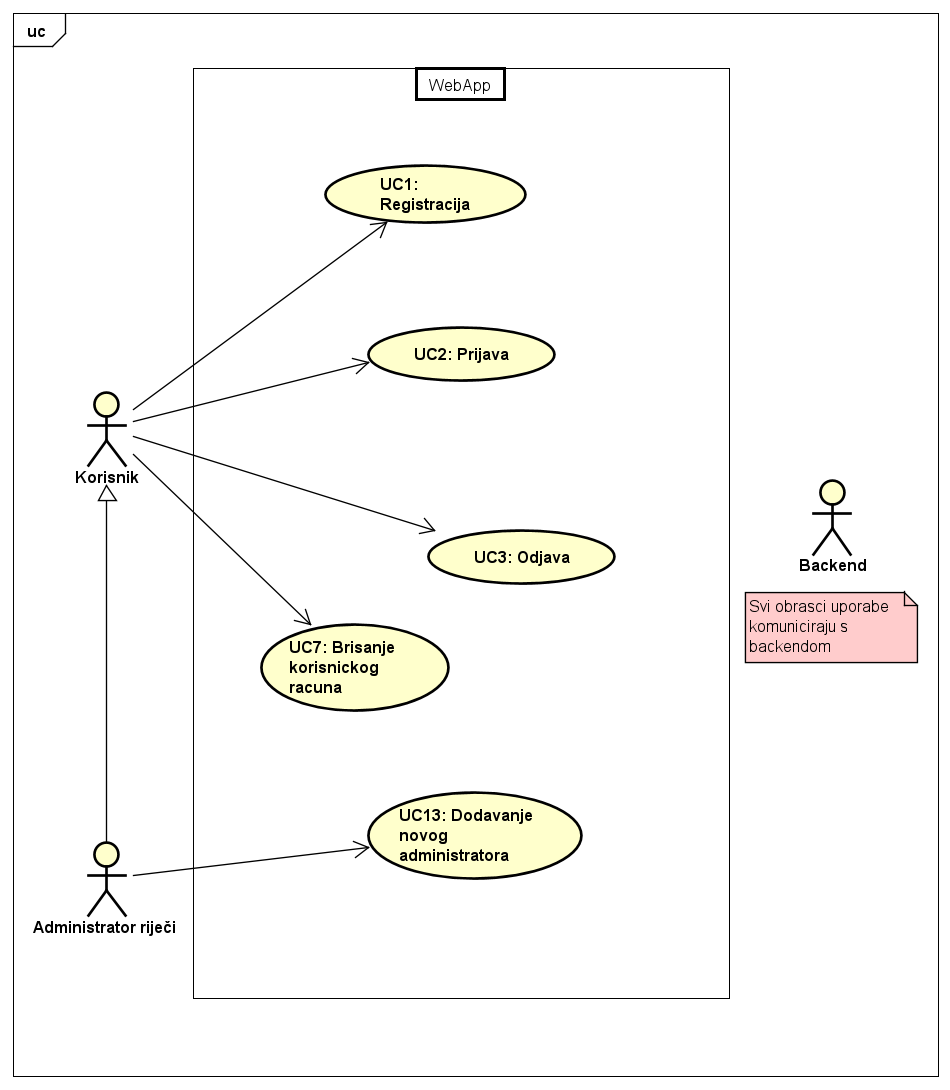
\includegraphics[width=\textwidth]{UseCaseDiagram0}
					Slika 3.1: Dijagram obrazaca uporabe, funkcionalnosti korisnika i administratora riječi
					
					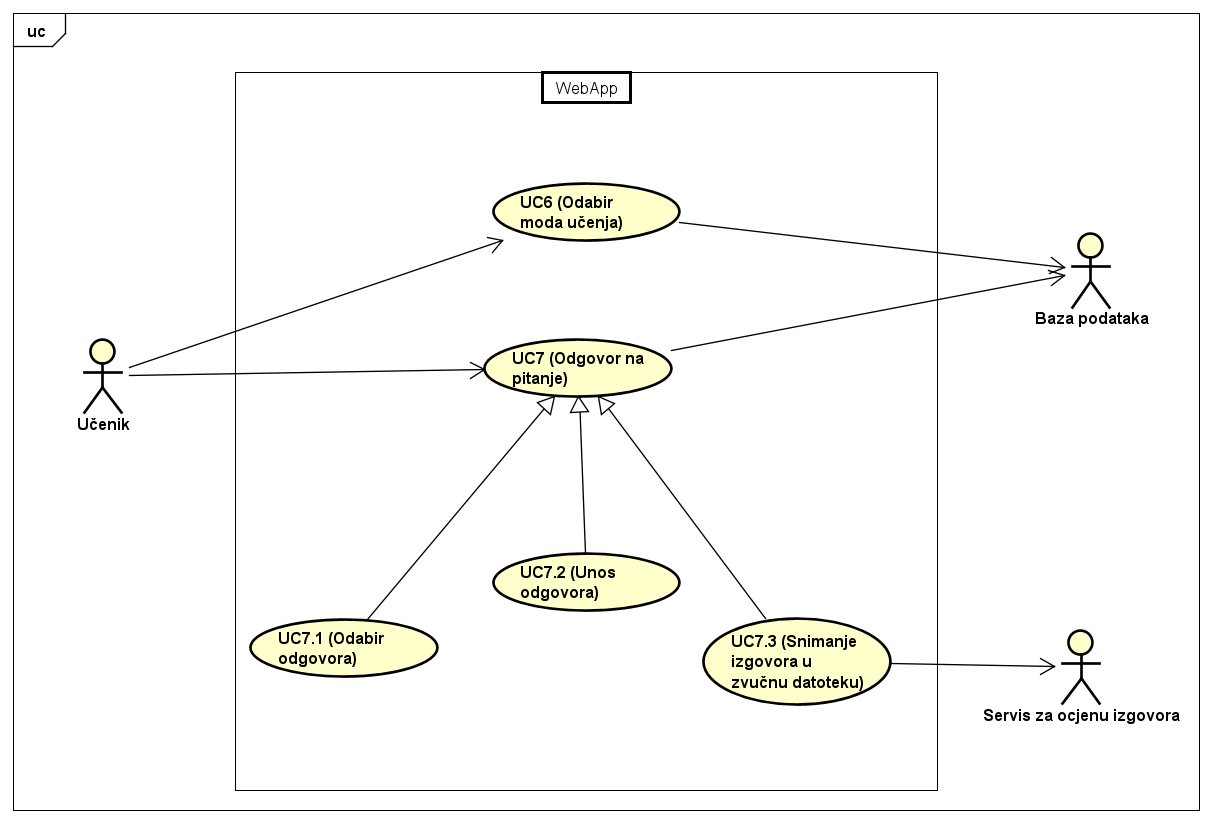
\includegraphics[width=\textwidth]{UseCaseDiagram1}
					Slika 3.2: Dijagram obrazaca uporabe, funkcionalnosti korisnika
					
					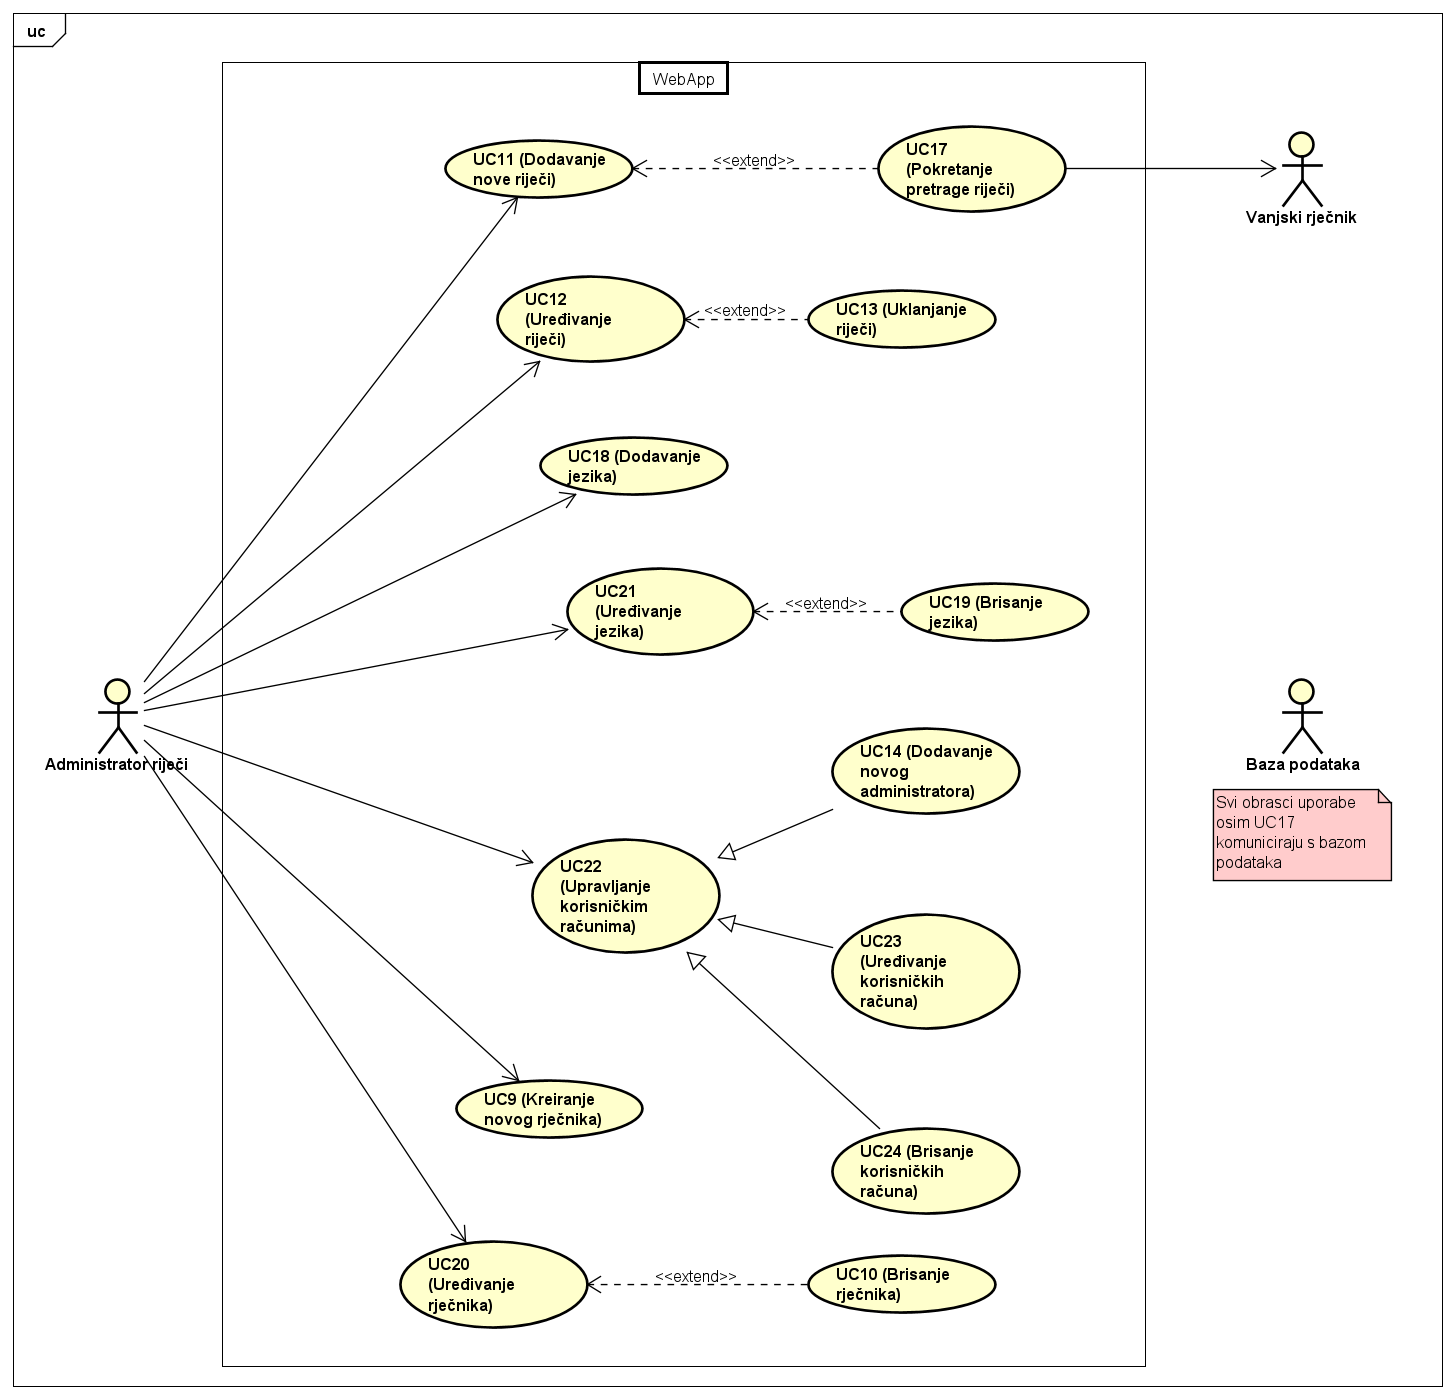
\includegraphics[width=\textwidth]{UseCaseDiagram2}
					Slika 3.3: Dijagram obrazaca uporabe, funkcionalnosti administratora riječi
				
			\subsection{Sekvencijski dijagrami}
				
%				\textbf{\textit{dio 1. revizije}}\\
%				
%				\textit{Nacrtati sekvencijske dijagrame koji modeliraju najvažnije dijelove sustava (max. 4 dijagrama). Ukoliko postoji nedoumica oko odabira, razjasniti s asistentom. Uz svaki dijagram napisati detaljni opis dijagrama.}
%				\eject
	
		\section{Ostali zahtjevi}
		
			\begin{packed_enum}
				
				\item Web app
				\item Koristi api za rijeci
				\item https
				\item Objektno orijentirani jezici
				\item Kriptirane lozinke
				\item Sustav jednostavan i intuitivan za korištenje
				\item Sustav podržava više korisnika istovremeno
				
			\end{packed_enum}
		
%			\textbf{\textit{dio 1. revizije}}\\
%		 
%			 \textit{Nefunkcionalni zahtjevi i zahtjevi domene primjene dopunjuju funkcionalne zahtjeve. Oni opisuju \textbf{kako se sustav treba ponašati} i koja \textbf{ograničenja} treba poštivati (performanse, korisničko iskustvo, pouzdanost, standardi kvalitete, sigurnost...). Primjeri takvih zahtjeva u Vašem projektu mogu biti: podržani jezici korisničkog sučelja, vrijeme odziva, najveći mogući podržani broj korisnika, podržane web/mobilne platforme, razina zaštite (protokoli komunikacije, kriptiranje...)... Svaki takav zahtjev potrebno je navesti u jednoj ili dvije rečenice.}
			 
			 
			 
	